\documentclass{article}
\setlength{\parskip}{5pt} % esp. entre parrafos
\setlength{\parindent}{0pt} % esp. al inicio de un parrafo
\usepackage{amsmath} % mates
\usepackage{listings}
\usepackage[sort&compress,numbers]{natbib} % referencias
\usepackage{url} % que las URLs se vean lindos
\usepackage[top=25mm,left=20mm,right=20mm,bottom=25mm]{geometry} % margenes
\usepackage{hyperref} % ligas de URLs
\usepackage{graphicx} % poner figuras
\usepackage[spanish]{babel} % otros idiomas
\usepackage{textcomp}
\usepackage{pgfplots} % crear graficas
\pgfplotsset{width=9cm,compat=1.7}
\title{"P2" Teoría de Colas} %Título
\author{NESTOR}
\date{Marzo 2022}

\begin{document} % inicia contenido

\maketitle % cabecera


 

\section{Objetivo}
El objetivo de la pr\'actica consiste en analizar los tiempos de ejecuci\'on de ("n") algoritmos de diferentes que se encuentran en un número entero dado que es un número primo. Ya que un número primo es un número natural mayor que ("1") que tiene únicamente dos divisores positivos distintos. Ya que que se trata de un número positivo que es imposible de expresar como producto de otros dos números enteros igualmente positivos pero menores que él o en su defecto como un producto de dos números enteros que poseen varias formas.

\section{Desarrollo}
De acuerdo con el desarrollo en el \href{https://github.com/satuelisa/Simulation/blob/master/QueuingTheory/ordering.py}{c\'odigo} implementado por E. Schaeffer \cite{elisa1}, primero se definen los parámetros de ejecución de los algoritmos, donde se crea una lista de n\'umeros desde 1000 hasta 7919. A continuación se muestra los siguientes comandos:

\begin{lstlisting}

from math import ceil, sqrt
from random import shuffle
import multiprocessing
from time import time
from scipy.stats import f_oneway
import pandas as pd
import matplotlib.pyplot as plt
import seaborn as sns

d = 1000
h = 7919 
replicas = 30
original = [x for x in range(d, h + 1)]
invertido = original[::-1]
aleatorio = original.copy()
shuffle(aleatorio)
cores = multiprocessing.cpu_count()

def primo_1(n):
if n < 3:
    return True
for i in range(2, n):
    if n % i == 0:
    return False
    return True

def primo_2(n):
if n < 4:
    return True
if n % 2 == 0:
    return False
for i in range(3, n - 1, 2):
    if n % i == 0:
    return False
    return True

def primo_3(n):
if n < 4:
    return True
if n % 2 == 0:
    return False
for i in range(3, int(ceil(sqrt(n))), 2):
    if n % i == 0:
    return False
    return True

def primo_4(n):
if n < 4:
    return True
if n % 2 == 0:
    return False
for i in range(4, int(ceil(sqrt(n))), 3):
    if n % i == 0:
    return False
    return True

if __name__ == "__main__":
resultados_1 = {'Prueba 1': [], 'Prueba 2': [], 'Prueba 3': [], 'Prueba 4': []}              
resultados_2 = {'Resultado 1': [], 'Resultado 2': [], 'Resultado 3': [], 'Resultado 4': []}
with multiprocessing.Pool(processes = cores-1) as pool:
  pool.map(primo_1, original)
  for r in range(replicas):
    t = (time()*1000)
    pool.map(primo_1, original)
    resultados_1['Prueba 1'].append((time()*1000)-t)
    t = (time()*1000)
    pool.map(primo_2, original)
    resultados_1['Prueba 2'].append((time()*1000)-t)
    t = (time()*1000)
    pool.map(primo_3, original)
    resultados_1['Prueba 3'].append((time()*1000)-t)
    t = (time()*1000)
    pool.map(primo_4, original)
    resultados_1['Prueba 4'].append((time()*1000)-t)
    t = (time()*1000)
    pool.map(primo_3, original)
    resultados_2['Resultado 1'].append((time()*1000) - t)
    t = (time()*1000)
    pool.map(primo_3, invertido)
    resultados_2['Resultado 2'].append((time()*1000) - t)
    t = (time()*1000)
    pool.map(primo_3, aleatorio)
    resultados_2['Resultado 3'].append((time()*1000) - t)
    t = (time()*1000)
    pool.map(primo_3, aleatorio)
    resultados_2['Resultado 4'].append((time()*1000) - t)
df1 = pd.DataFrame(data = resultados_1)
df2 = pd.DataFrame(data = resultados_2)
print(df1, '\n', df2)
stat1, p1 = f_oneway(resultados_1['Prueba 1'],
    resultados_1['Prueba 2'],
    resultados_1['Prueba 3'],
    resultados_1['Prueba 4'])
print('Variando algoritmo\n', 'stat=%.3f, p=%.3f' % (stat1, p1))
if p1 > 0.05: print('Estadísticamente no significativa\n')
else:
print('Estadísticamente significativa\n')
    stat2, p2 = f_oneway(resultados_2['Resultado 1'],
    resultados_2['Resultado 2'],
    resultados_2['Resultado 3'],
    resultados_2['Resultado 4'])
print('Variando orden de numeros\n', 'stat=%.3f, p=%.3f' % (stat2, p2))
if p2 > 0.05:
 print('Estadísticamente no significativa\n')
else:
 print('Estadísticamente significativa\n')
    
    sns.violinplot(data = df1, scale='count')
    plt.savefig('Prueba.png')
    plt.show()
    sns.violinplot(data = df2, scale='count')
    plt.savefig('Resultado.png')
    plt.show()
    
    
\end{lstlisting}


\section{Resultados}
Se muestra en las gráficas para visualizar la distribución de los datos y su densidad de probabilidad. Este gráfico es una combinación de un diagrama de cajas y bigotes y un diagrama de densidad girado y colocado a cada lado, para mostrar la forma de distribución de los datos. La barra negra gruesa en el centro representa el intervalo intercuartil, la barra negra fina que se extiende desde ella, representa el 95 por ciento de los intervalos de confianza, y el punto blanco es la mediana. A continuación se muestra las siguiemtes gráficas:


\newpage
\begin{figure_1}
    \centering
    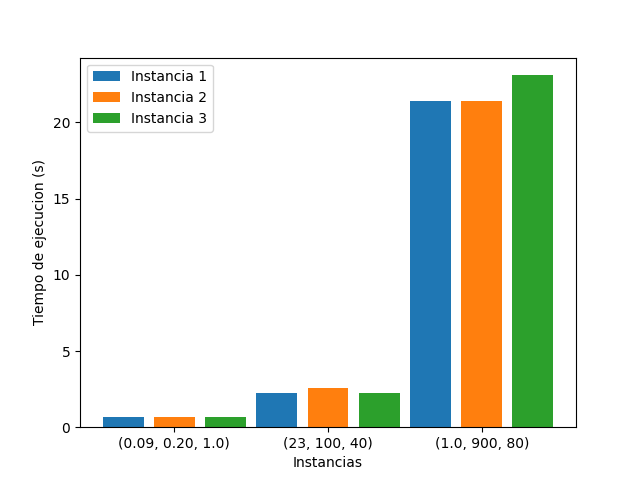
\includegraphics[width=170mm]{Figure_1.png}
    \caption{Figura 1: Prueba de Algoritmo}
    \label{figure_1}

\begin{figure_2}
    \centering
    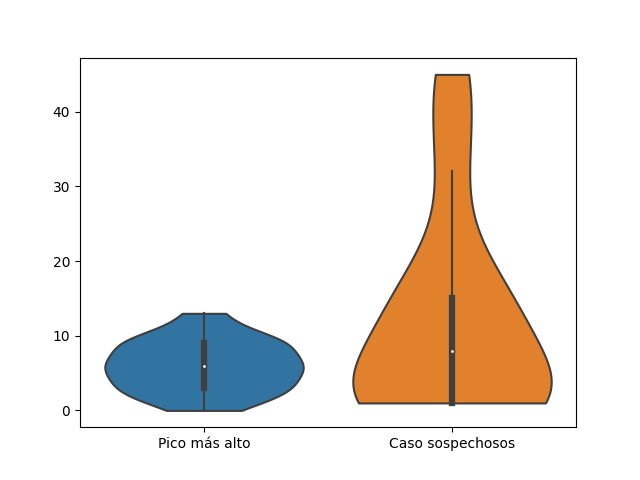
\includegraphics[width=170mm]{Figure_2.png}
    \caption{Figura 2: Resultado de Variación}
    \label{figure_2}
\end{figure_2}



\section{Conclusiones}

Como puede verse en la tabla, tenemos una densidad más alta entre 100 y 300 para la figura 1 y para la figura 2 es de 5 y 10. Eso es muy significativo porque, como en la descripción nos da un valor medio.


\bibliography{simulacion}
\cite{jorge}
\cite{elisa1}
\cite{natalia}
\cite{Denisse}
\cite{Matpltlib}
\bibliographystyle{plain}
\end{document}
